% figures/layer_distribution.tex -- Layer distribution: IOI vs Multi-step
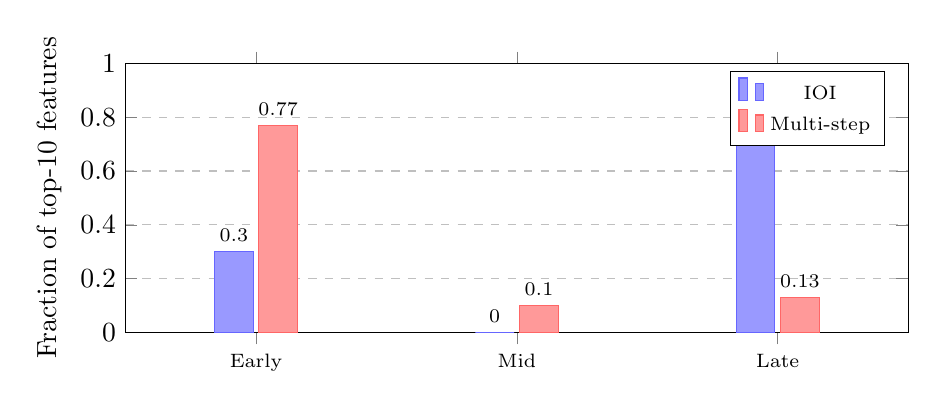
\begin{tikzpicture}
\begin{axis}[
    ybar,
    width=0.95\columnwidth,
    height=5cm,
    bar width=14pt,
    enlarge x limits=0.25,
    ylabel={Fraction of top-10 features},
    symbolic x coords={Early, Mid, Late},
    xtick=data,
    x tick label style={font=\scriptsize},
    ymin=0, ymax=1.0,
    ytick={0, 0.2, 0.4, 0.6, 0.8, 1.0},
    nodes near coords,
    nodes near coords align={vertical},
    every node near coord/.append style={font=\scriptsize},
    legend style={at={(0.97,0.97)}, anchor=north east, font=\scriptsize},
    ymajorgrids=true,
    grid style=dashed,
]

% IOI (late-layer dominant: top features in L24, L25, L6, L8)
\addplot[fill=blue!40, draw=blue!60] coordinates {
    (Early, 0.30) (Mid, 0.0) (Late, 0.70)
};

\addplot[fill=red!40, draw=red!60] coordinates {
    (Early, 0.77) (Mid, 0.10) (Late, 0.13)
};

\legend{IOI, Multi-step}
\end{axis}
\end{tikzpicture}
